\documentclass[12pt, twoside]{article}
% \documentclass[12pt, twoside]{article}
\usepackage[letterpaper, margin=1in, headsep=0.2in]{geometry}
\setlength{\headheight}{0.6in}
%\usepackage[english]{babel}
\usepackage[utf8]{inputenc}
\usepackage{microtype}
\usepackage{amsmath}
\usepackage{amssymb}
%\usepackage{amsfonts}
\usepackage[nomessages]{fp} %\FPeval{\var-name}{2*sin(pi/6)}
\usepackage{siunitx} %units in math. eg 20\milli\meter
\usepackage{yhmath} % for arcs, overparenth command
\usepackage{tikz} %graphics
\usetikzlibrary{quotes, angles, arrows, arrows.meta}
\usepackage{graphicx} %consider setting \graphicspath{{images/}}
\usepackage{parskip} %no paragraph indent
\usepackage{enumitem}
\usepackage{multicol}
\usepackage{venndiagram}

\usepackage{fancyhdr}
\pagestyle{fancy}
\fancyhf{}
\renewcommand{\headrulewidth}{0pt} % disable the underline of the header
\raggedbottom
\hfuzz=2mm %suppresses overfull box warnings

\usepackage{hyperref}
\usepackage{float}

\title{Algebra 2}
\author{Chris Huson}
\date{October 2023}

\fancyhead[LE]{\thepage}
\fancyhead[RO]{\thepage \\ First and last name: \hspace{2.5cm} \,\\ Section: \hspace{2.5cm} \,}
\fancyhead[LO]{BECA / Huson / Algebra 2: Polynomials \\* 2 October 2024}

\begin{document}

\subsubsection*{2.8 Homework: Operations on polynomials}
\begin{enumerate}

\item Simplify the sum of these two polynomials: $(3x^3+5x^2+x+6)+(x^3-2x^2+7x-8)$ \vspace{2cm}

\item Given the two functions $f(x)=5x^3+8x^2-x$ and $g(x)=x^4+2x^3+x^2-5$, find their difference $f(x)-g(x)$ as a polynomial in standard form. \vspace{3cm}

\item Multiply the two polynomials $f(x)=2x+5$ and $g(x)=2x^2+3x-1$. First complete the grid and then collect terms to find the product as a polynomial in standard form. \\[0.25cm]
\begin{tabular}{|p{1cm}|p{3cm}|p{3cm}|p{3cm}|}
    \hline
     & $2x^2$ & $+3x$ & $-1$ \\
    \hline
    $2x$ &  & & \\[0.5cm]
    \hline
    $+5$ &  & & \\[0.5cm]
    \hline
\end{tabular} \vspace{4cm}

\item Using subscript notation, write a recursive formula for the sequence $5, 10, 20, 40, 80, 160, \dots$ \vspace{2cm}

\item Using subscript notation, write a recursive formula for the sequence $11, 3, -5, -13, \dots$ 

\newpage
\item Select all of the expressions that are equivalent to $x^2-7x+12$.
    \begin{multicols}{2}
    \begin{enumerate}
        \item $(x-2)(x-6)$
        \item $(x-6)(x-2)$ 
        \item $(x+4)(x+3)$ 
        \item $(x-3)(x-4)$ 
        \item $(x-4)(x+3)$
        \item $(x+3)(x+4)$ 
        \item $(x-4)(x-3)$
        \item $x^2+7x-12$
    \end{enumerate} 
    \end{multicols}
    \vspace{0.25cm}

\item Select all solutions to the equation $(2x-1)(x+5)=0$.
    \begin{multicols}{2}
    \begin{enumerate}
        \item $x=0.5$
        \item $x=-5$
        \item $x=2.5$
        \item $x=-0.5$
        \item $x=5$
        \item $x=\frac{1}{2}$
    \end{enumerate}
    \end{multicols}
    \vspace{0.25cm}

\item Here is the graph of a quadratic function. Which of the following could be its equation?
    \begin{center}
    \begin{tikzpicture}[xscale=0.5, yscale=0.25]
        \draw [thick, ->] (-4.2,0) -- (6.4,0) node [above] {$x$};
        \draw [thick, ->] (0,-9.2)--(0,9.5) node [right] {$y$};
        \foreach \x in {-4,-2,2,4,6} \draw (\x cm,4pt) -- (\x cm,-4pt) node[below] {$\x$};
        \foreach \y in {-8,-4,4, 8} \draw (2pt,\y cm) -- (-2pt,\y cm) node[left] {$\y$};
        %\fill (-1,0) circle[radius=0.1] node[above left]{$j$};
        %\fill (3,0) circle[radius=0.1] node[above right]{$k$};
        \draw [thick, <->,smooth,samples=20,domain=-3:5] plot(\x,\x*\x-2*\x-8);
    \end{tikzpicture}
    \end{center}
    \begin{multicols}{2}
    \begin{enumerate}
        \item $y=(x+2)(x-4)$
        \item $y=(x-2)(x+4)$
        \item $y=(x+2)(x+4)$
        \item $y=(x-2)(x-4)$
    \end{enumerate}
    \end{multicols}

\item Find all of the solutions to the equation $x(x-11)(3x-8)(x+3)=0$. 

\newpage
\item Without a calculator, evaluate each polynomial for the given value of $x$.
\begin{multicols}{2}
    \begin{enumerate}[itemsep=1cm]
        \item $f(x)=-x^3+12x^2-x+4$, $x=1$ \\[0.25cm] 
        $f(1) = $ \vspace{2cm}
        \item $g(x)=x^4+x^3+x^2$, $x=-1$ \\[0.25cm] 
        $g(-1) = $ \vspace{2cm}
    \end{enumerate}
    \end{multicols}

\item Use a calculator to find the value of $h(x)=2x^3-3x^2+5x+2$ for $x=-3$. \\[0.25cm] 
$h(-3) = $ \vspace{2cm}

\item A polynomial $A$ is used to model the value of an investment account. Two deposits were made which earned interest annually.  $$A(x)=150x^4+300x^2$$ 
\begin{enumerate}[itemsep=1cm]
    \item The first deposit of \$150 was made four years ago. How much was the second deposit, and how long ago was it made? \vspace{2cm}
    \item Find the value of $A(x)$ for $x = 1.05$ to the \emph{nearest cent}. \vspace{2cm}
    \item If the interest rate earned on the account is $r = 7 \frac{1}{2}\%$ what value of $x$ would be used in the formula? \vspace{2cm}
\end{enumerate}

\end{enumerate}
\end{document}